\documentclass[amsmath,amssymb,notitlepage,11pt]{revtex4}
%\documentclass[12pt]{article}
\usepackage[toc,page]{appendix}
\usepackage{graphicx}
\usepackage{bm}% bold math
\usepackage{multirow}
\usepackage{booktabs}
\usepackage{verbatim}
\usepackage{hyperref}
\usepackage{enumitem}
\hypersetup{pdftex,colorlinks=true,allcolors=blue}
\usepackage{hypcap}
\usepackage[small,compact]{titlesec}
\setlist[enumerate]{itemsep=0mm}
%\addtolength{\textwidth}{1cm}
%\addtolength{\hoffset}{-0.5cm}
\addtolength{\textheight}{1.0cm}
\addtolength{\voffset}{-0.5cm}
\begin{document}
\title{CLAS12 M{\o}ller Operations Manual - v0.0}
\date{\today}
\author{N. Baltzell}
\begin{abstract}
\end{abstract}

\maketitle
%\tableofcontents
%\newpage

\section{Introduction}
The CLAS12 M{\o}ller system measures the polarization of the electron beam delivered to Hall B, and this document details its operating procedures.  The user interface for shift workers is shown in Fig.~\ref{fig:unconfig} and provides direct access to all controls and feedback that the normal operator should need, described in Section~\ref{sec:user}.  Expert operations are described in Section~\ref{sec:expert}.

\begin{figure}[htbp]\centering
    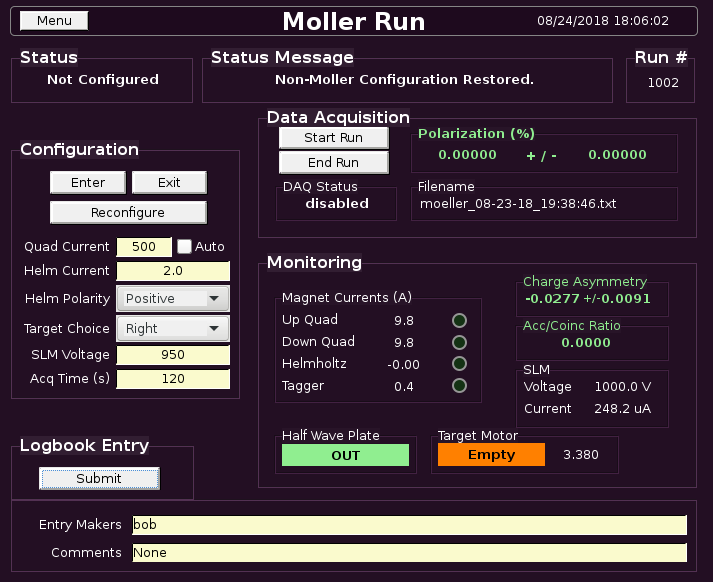
\includegraphics[width=11cm]{pics/unconfig}
    \caption{The user interface for shift workers for operating a M{\o}ller run is divided into status, configuration, data acquisition, monitoring, and logbook sections.  In this screenshot, the Moller symstem is not configured, i.e. the setup is for non-M{\o}ller beam delivery.\label{fig:unconfig}}
\end{figure}

\section{Standard Procedures}\label{sec:user}
The procedure for the operator can be summarized in the following steps, and more details are shown on the next page.
\begin{enumerate}
\vspace{-4mm}\item {\bf Configure}:  ensure the Configuration section is set as desired
\vspace{-4mm}\item {\bf Enter}: click {\em Enter} in the Configuration section and wait for success status
\vspace{-4mm}\item {\bf Start Run}: click {\em Start Run} in the DAQ section
\vspace{-4mm}\item {\bf Monitor}: monitor the critical parameters
\vspace{-4mm}\item {\bf End Run}: click {\em End Run} in the DAQ section
\vspace{-4mm}\item {\bf Log Entry}: click {\em Submit} in the Logbook Entry section 
\vspace{-4mm}\item {\bf Exit}: click {\em Exit} in the Configuration section and wait for success status
\end{enumerate}

\begin{enumerate}
\item {\bf Configure}:  ensure the Configuration section is set as desired
        \subitem
        The operator should confirm the desired values in the Configuration section.  This includes quadrupole current, Helmholtz current and polarity, target choice, SLM voltage, and acquisition time.  If the {\em Auto} option is selected for the quadrupoles, their current will be chosen based on standard settings for the current beam energy.  {\em Note, it is critical that some of these settings are held fixed while a run is ongoing, and those cannot be changed during a run from this interface.  See below regarding reconfiguring.}
\item {\bf Enter}: click {\em Enter} in the Configuration section and wait for success status
    \subitem Clicking the {\em Enter} button will configure the system for a M{\o}ller run by initiating a sequence of actions and provide corresponding feedback in the status portion of the screen.  This includes turning off some detectors' high voltage, energizing the quadrupoles and Helmholtz magnets, and inserting the M{\o}ller target.  Success will result in ``Moller Configuration Ready'' in the status message.
\item {\bf Start}: click {\em Start Run} in the DAQ section
    \subitem This will initiate a new M{\o}ller run, including zeroing any accumulated data, opening a new data file, incrementing the run number, and starting recording data.
\item {\bf Monitor}: monitor the critical parameters
    \subitem This is left to the operator.  The polarization and its uncertainty, the beam charge asymmetry, and the accidential-coincidence ratio should be in acceptable ranges.
\item {\bf End}: click {\em End Run} in the DAQ section
\item {\bf Log}: click {\em Submit} in the Logbook Entry section 
    \subitem This will submit a log entry to HBLOG with a table summarizing the results and an attached data file. {\em Note, at the point you may wish to navigate to the log entry in a web browser and add any relevant screenshots as comments to the entry}.
\item {\bf Reconfigure (optional)} At this point you can reconfigure, e.g. change the Helmholtz polarity by adjusting the configuration and and clicking {\em Reconfigure}, and then click {\em Start Run}.
\item {\bf Exit}: click {\em Exit} in the Configuration section and wait for success status
    \subitem  This will restore the non-M{\o}ller configuration by turning of the quadrupoles and Helmholtz and retracting the M{\o}ller target.  {\em Note, it will not restore any detector high voltage}. 
\end{enumerate}

\subsection{Status Values}
Describe the possible values of the status variable in the top left of the screen.

\section{Expert Procedures}\label{sec:expert}
The instructions for the old, manual procedure.

\begin{appendices}
Description of the hardware and software involved in the CLAS12 M{\o}ller system.
\subsection{Quadrupoles}
\subsection{Helmholtz}
\subsection{Synchrotron Light Monitor}
\subsection{Target}
\subsection{Helicity Signal}
\subsection{Multi-Channel Scaler}
\subsection{EPICS IOCs}
\end{appendices}

\end{document}

